\documentclass[10pt,a4paper]{article}
\usepackage[a4paper,margin=2cm]{geometry}
\usepackage{fontspec}
\IfFontExistsTF{Arial}{\setmainfont{Arial}}{\setmainfont{TeX Gyre Heros}}
\IfFontExistsTF{Consolas}{\setmonofont[Scale=0.9]{Consolas}}{}
\usepackage{microtype}
\usepackage{graphicx,booktabs,tabularx,array}
\usepackage[font=small,labelfont=bf,skip=4pt]{caption}
\usepackage{enumitem}
\setlist{nosep,leftmargin=1.4em}
\usepackage{titlesec}
\titleformat{\section}{\large\bfseries}{\thesection}{0.6em}{}
\titlespacing*{\section}{0pt}{9pt}{3pt}
\titleformat{\subsection}{\normalsize\bfseries}{\thesubsection}{0.6em}{}
\titlespacing*{\subsection}{0pt}{6pt}{2pt}
\setlength{\parindent}{0pt}
\setlength{\parskip}{4pt}
\setlength{\tabcolsep}{3.5pt}
\setlength{\textfloatsep}{8pt plus 2pt minus 2pt}
\setlength{\floatsep}{6pt plus 2pt minus 2pt}
\setlength{\intextsep}{6pt plus 2pt minus 2pt}
\usepackage{csquotes}
\usepackage[backend=biber,style=ieee,sorting=none,url=false,isbn=false]{biblatex}
\addbibresource{references.bib}
\usepackage[hidelinks]{hyperref}
\usepackage{xcolor}
% A section another member still has to write; delete the box when it is done.
\newcommand{\placeholder}[1]{\par\noindent\fcolorbox{orange}{orange!8}{%
  \parbox{\dimexpr\linewidth-2\fboxsep-2\fboxrule\relax}{\small #1}}\par}
\begin{document}

\begin{titlepage}
\centering
\vspace*{3.5cm}
{\LARGE\bfseries Do ECG Heartbeat Classifiers Generalise to Unseen Patients?\par}
\vspace{0.4cm}
{\Large A Controlled Study of a 1D CNN on MIT-BIH\par}
\vspace{2cm}
{\large SC4001 Neural Networks and Deep Learning: Group Project Report\par}
\vspace{0.6cm}
{\large\bfseries Group [number]\par}
\vspace{1.2cm}
Huang Yitian: evaluation and report (M3)\par\vspace{0.15cm}
[M1 full name]: data and features (M1)\par\vspace{0.15cm}
[M2 full name]: models and training (M2)\par\vspace{0.15cm}
\vfill
November 2026
\end{titlepage}
\setcounter{page}{1}

\section{Introduction}

Automatic heartbeat classification from the electrocardiogram (ECG) supports long-term monitoring, where a single day of recording contains around 100,000 beats. The MIT-BIH Arrhythmia Database~\cite{Moody2001,Goldberger2000} is the standard benchmark, with beats grouped into the AAMI classes normal (N), supraventricular ectopic (S), ventricular ectopic (V), fusion (F) and unknown (Q)~\cite{AAMI2012}.

Reported results depend heavily on how beats are split. If beats from all recordings are pooled and divided at random (the \emph{intra-patient} paradigm), beats from the same person appear in both the training and the test set, so a model can succeed by recognising the person rather than the arrhythmia. Under this paradigm deep models report near-perfect scores, for example 100\% S sensitivity at 96.5\% positive predictivity~\cite{Mousavi2019}. When training and test recordings are disjoint (the \emph{inter-patient} split of de Chazal et al.~\cite{dechazal2004automatic}) the task is much harder: their classifier found 75.9\% of S beats at a positive predictivity of only 38.5\%, and Sellami and Hwang report 99.48\% accuracy intra-patient but 88.34\% inter-patient~\cite{Sellami2019}. The same pattern appears across clinical machine learning: record-wise validation often overestimates accuracy compared with subject-wise validation~\cite{Saeb2017}, and leakage between training and test data has produced over-optimistic conclusions in many fields~\cite{Kapoor2023}. A deployed classifier always meets a new patient, so only a patient-wise evaluation answers the clinically relevant question.

The patient-wise benchmark has a difficulty of its own: abnormal beats are rare and concentrated in a few people. In the standard test set (DS2; 49,661 beats after our preprocessing) S beats make up 3.7\% of beats, and one recording, 232, contains 75\% of them; recording 213 contains 93\% of the test F beats. Predicting N for every beat already scores 89.0\% accuracy, with a macro-F1 of only 0.24.

This project asks \textbf{how much a 1D convolutional neural network (CNN) loses when it is evaluated on patients it has never seen, and whether inexpensive changes recover the rare abnormal classes.} We train one baseline on a random beat split and on a subject-disjoint patient split, and then test four changes, each aimed at a suspected cause of the gap: class-weighted and focal losses for class imbalance~\cite{Cui2019,Lin2017}, waveform augmentation for differences in recording conditions~\cite{Um2017,Iwana2021}, and RR-interval features, because S beats are mostly early relative to the local rhythm while their shape resembles that of N beats. Our contributions are:

{\begin{itemize}
\item A controlled measurement of the gap: macro-F1 falls from 0.874 to 0.429, and S and F F1 fall from 0.74 and 0.81 to zero. Our patient split is fully subject-disjoint; records 201 and 202 come from the same person, which the conventional split ignores.
\item A comparison of four fixes over three seeds, with per-class sensitivity, positive predictivity and F1, per-patient results and patient-bootstrap intervals. None recovers S detection; class weighting appears to, but only by labelling whole patients as S.
\item A failure analysis showing that RR features teach the network to rank S beats correctly \emph{within} a patient (AUROC 0.994 in record 232) even though it never predicts S, and that a decision threshold set on other patients does not fix this.
\item A data analysis explaining why timing does not transfer: 62\% of training S beats lie inside tachycardia runs, where they are not early, while most test S beats are isolated early beats.
\end{itemize}\par}

\section{Review of Existing Techniques}

\subsection{Heartbeat classification on MIT-BIH}

\placeholder{\textbf{[M2 to write: 2.1 Heartbeat classification on MIT-BIH and class imbalance, about 300 words.]} MIT-BIH and the DS1/DS2 inter-patient protocol, feature-based and deep classifiers, and class imbalance with its loss-based remedies (weighted and focal loss, which E2 and E3 test). Verified sources: \texttt{docs/report/REFERENCES\_VERIFIED.md}; an earlier starting text is in \texttt{docs/report/M3\_RELATED\_WORK.md} (2.1).}

\subsection{Timing features and data augmentation}

\placeholder{\textbf{[M1 to write: 2.2 Timing features and data augmentation, about 150 words.]} Source: the integration-ready paragraph in \texttt{docs/report/M1\_RELATED\_WORK.md}.}

\subsection{Evaluation protocols and patient-level uncertainty}

An evaluation is only meaningful if the relationship between training and test data matches that between training data and future use~\cite{Saeb2017}. Even the conventional inter-patient split is not fully subject-disjoint: records 201 (DS1) and 202 (DS2) come from the same person, and PhysioNet advises keeping them in one partition for subject-independent work~\cite{moody2005mitbih}. How results are summarised also matters. ANSI/AAMI EC57 emphasises record-by-record reporting~\cite{AAMI2012}, yet headline inter-patient results are single figures per class, pooled over DS2. Such pooled figures are dominated by a few recordings, and beats from one patient are not independent, so intervals that treat beats as independent samples are too narrow. Resampling whole clusters, here patients, is the standard bootstrap for clustered data~\cite{Field2007,Davison1997,Efron1993}. We therefore report per-record results, results without the dominant records, and patient-bootstrap intervals alongside the pooled metrics.

\section{Data and Methods}

\subsection{Data and preprocessing}

\placeholder{\textbf{[M1 to write: 3.1 Data and preprocessing.]} Source: “Data and preprocessing” in \texttt{docs/report/M1\_REPORT\_INSERT.md} (records used, class mapping, beat windows, 100,630 beats, training-only standardisation).}

\subsection{Partitions}

\placeholder{\textbf{[M1 to write: 3.2 Partitions, with a table of beats per partition and class.]} Source: “Partitions and timing features” in \texttt{docs/report/M1\_REPORT\_INSERT.md}. The main E1–E5 protocol is \texttt{patient\_strict} (record 201 removed from training: 17 training, 4 validation and 22 test subjects); E0 uses the random split.}

\subsection{RR features and augmentation}

\placeholder{\textbf{[M1 to write: 3.3 RR features (E5) and augmentation (E4).]} Source: \texttt{docs/report/M1\_REPORT\_INSERT.md}. Section 4.4 uses the fourth RR feature (previous RR divided by the mean of the last ten) as the \emph{prematurity index}, so please name it here.}

\subsection{Model and training}

\placeholder{\textbf{[M2 to write: 3.4 Model and training, about 200 words.]} The CNN architecture and parameter count, the optimiser and early-stopping settings actually used (30 epochs, patience 4, not the script defaults), the E2 class weights and the E3 focal loss, and the seeds and hardware. The facts are listed in \texttt{docs/report/M3\_RESULTS.md} §4.1.}

\subsection{Evaluation}

Abnormal beats are concentrated in a few records (Fig.~\ref{fig:1}): record 209 holds 60\% of the training S beats and record 208 holds 94\% of the training F beats, while in the test set record 232 holds 75\% of the S beats and record 213 holds 93\% of the F beats. Pooled test scores therefore mostly describe a few patients, and our evaluation is designed around this.

\begin{figure}[!htb]
\centering
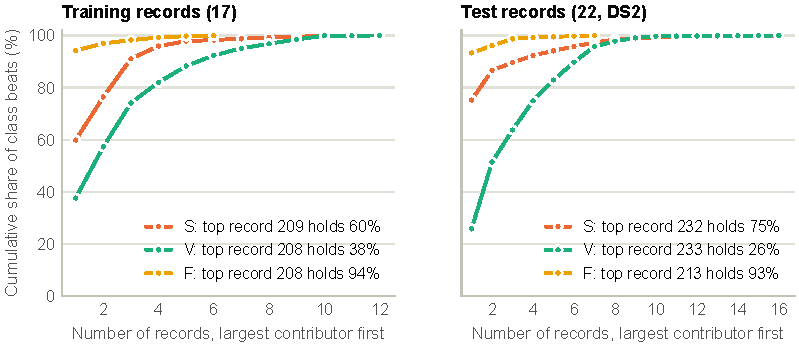
\includegraphics[width=6.0in]{figures/class_concentration.pdf}
\caption{Concentration of abnormal beats: cumulative share of each class's beats, records sorted by contribution. Left: the 17 training records; right: the 22 test records.}\label{fig:1}
\end{figure}

We report per-class sensitivity (Se, recall), positive predictivity (+P, precision) and F1, and the macro-F1 over the four classes, as mean\,±\,SD over the three seeds. Test predictions were exported once from the frozen checkpoints. Before any test beat was read, the processed arrays passed the data audit and every checkpoint reproduced its stored validation macro-F1 on our copy of the data (largest difference 3 × 10$^{-4}$, from GPU/CPU rounding). Because two records dominate the test S and F beats, we also report S without record 232 and F without record 213 as sensitivity analyses. To show how much a result depends on which patients are tested, we resampled the 22 test records with replacement 2,000 times, using the same draws for every model, and report 95\% percentile intervals for each metric and for its paired difference from E1.

\section{Experiments and Results}

\subsection{Experiments and hypotheses}

E0 (random split) and E1 (patient split) use the baseline CNN with cross-entropy. E2–E5 each change one element relative to E1: class-weighted loss (E2), focal loss (E3), augmentation (E4) and RR features (E5). Before any training run, we wrote down five hypotheses: the gap is large and concentrated in S and F (H1); weighted and focal losses raise rare-class sensitivity at the cost of +P (H2); augmentation helps little (H3); RR features give the largest S gain (H4); and no conclusion about F will be robust (H5). A sixth hypothesis, on autoencoder pretraining (E6), was not tested: M1 pretrained the encoders, but no supervised E6 classifier was trained (Appendix B). Two analyses in Section 4.4 were added after the first test evaluation and are marked \emph{post-hoc}; no model or threshold was selected on test data.

\subsection{The generalisation gap (H1: supported)}

\begin{table}[!htb]
\centering\small
\caption{Main results on the full test set (mean\,±\,SD over three seeds). n/a: the class was never predicted. \textsuperscript{*}Only one seed predicted any S beat.}\label{tab:2}
\begin{tabularx}{\linewidth}{l>{\raggedright\arraybackslash}Xllllll}
\toprule
\textbf{Exp} & \textbf{Model (test set)} & \textbf{Macro-F1} & \textbf{S Se} & \textbf{S +P} & \textbf{S F1} & \textbf{V F1} & \textbf{F F1} \\
\midrule
— & always predict N (patient) & 0.236 & 0 & n/a & 0 & 0 & 0 \\
E0 & baseline (random split) & 0.874\,±\,0.009 & 0.618\,±\,0.027 & 0.910\,±\,0.017 & 0.736\,±\,0.023 & 0.955\,±\,0.005 & 0.814\,±\,0.010 \\
E1 & baseline (patient) & 0.429\,±\,0.002 & 0.000\,±\,0.000 & n/a & 0.000\,±\,0.000 & 0.756\,±\,0.008 & 0.000\,±\,0.000 \\
E2 & + weighted loss & 0.371\,±\,0.067 & 0.830\,±\,0.060 & 0.115\,±\,0.013 & 0.201\,±\,0.018 & 0.629\,±\,0.102 & 0.004\,±\,0.002 \\
E3 & + focal loss & 0.444\,±\,0.017 & 0.000\,±\,0.000 & n/a & 0.000\,±\,0.000 & 0.811\,±\,0.067 & 0.001\,±\,0.002 \\
E4 & + augmentation & 0.433\,±\,0.017 & 0.000\,±\,0.000 & n/a & 0.000\,±\,0.000 & 0.771\,±\,0.061 & 0.001\,±\,0.003 \\
E5 & + RR features & 0.445\,±\,0.030 & 0.001\,±\,0.001 & 0.167\textsuperscript{*} & 0.001\,±\,0.002 & 0.799\,±\,0.092 & 0.027\,±\,0.047 \\
\bottomrule
\end{tabularx}
\end{table}

The same network that reaches macro-F1 0.874 on a random beat split reaches 0.429 on unseen patients (Table~\ref{tab:2}, Fig.~\ref{fig:2}). Accuracy hides this: it falls only from 0.980 to 0.923, 3.3 points above the 0.890 of always predicting N. As H1 predicted, the loss is concentrated in the rare classes. S F1 falls from 0.736 to 0 and F F1 from 0.814 to 0, while V F1 falls less, from 0.955 to 0.756. On unseen patients the baseline never predicts S: 98.6\% of the 1,836 test S beats are called N, and the F beats of record 213 are split evenly between N and V.

\begin{figure}[!htb]
\centering
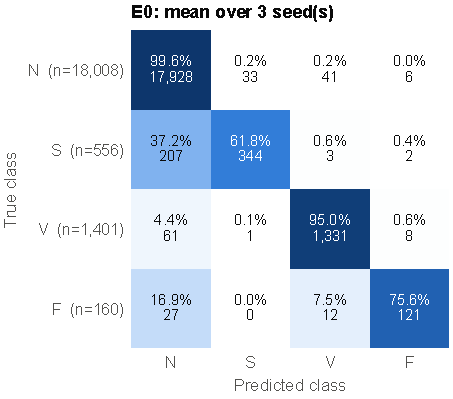
\includegraphics[width=3.0in]{figures/confusion_E0.pdf}\hspace{0.15in}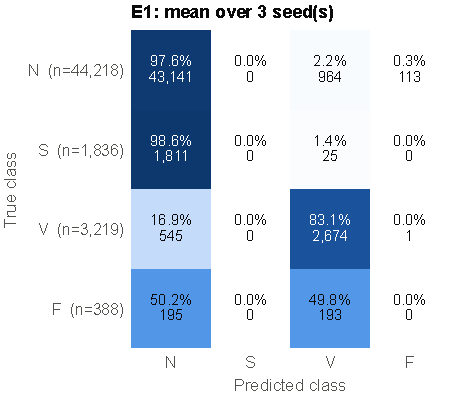
\includegraphics[width=3.0in]{figures/confusion_E1.pdf}
\caption{Confusion matrices of the same CNN on a random beat split (E0, left) and on unseen patients (E1, right), mean over three seeds. Cells show the percentage of the true class and the number of beats.}\label{fig:2}
\end{figure}

\subsection{Effect of the fixes (H2–H5)}

\begin{table}[!htb]
\centering\small
\caption{Change from E1 with 95\% patient-bootstrap intervals (2,000 resamples of the 22 test records, seed-averaged), and S and F F1 without their dominant records.}\label{tab:3}
\begin{tabularx}{\linewidth}{l>{\raggedright\arraybackslash}X>{\raggedright\arraybackslash}X>{\raggedright\arraybackslash}X>{\raggedright\arraybackslash}Xll}
\toprule
\textbf{Exp} & \textbf{Δ Macro-F1} & \textbf{Δ S F1} & \textbf{Δ V F1} & \textbf{Δ F F1} & \textbf{S F1 without 232} & \textbf{F F1 without 213} \\
\midrule
E2 & −0.058 [−0.135,~+0.042] & +0.201 [+0.008,~+0.473] & −0.127 [−0.227,~+0.016] & +0.004 [0.000,~+0.017] & 0.027\,±\,0.009 & 0.001\,±\,0.001 \\
E3 & +0.015 [−0.001,~+0.034] & 0 & +0.056 [−0.006,~+0.126] & +0.001 [0.000,~+0.020] & 0 & 0.002\,±\,0.003 \\
E4 & +0.004 [−0.003,~+0.016] & 0 & +0.015 [−0.014,~+0.049] & +0.001 [0.000,~+0.051] & 0 & 0.008\,±\,0.013 \\
E5 & +0.016 [+0.004,~+0.053] & +0.001 [0.000,~+0.012] & +0.043 [+0.012,~+0.079] & +0.027 [0.000,~+0.172] & 0.006\,±\,0.010 & 0.001\,±\,0.001 \\
\bottomrule
\end{tabularx}
\end{table}

{\begin{itemize}
\item \textbf{H2, partly supported.} Class weighting (E2) raises S sensitivity from 0 to 0.83, but S +P is 0.115, so about eight of every nine S predictions are false; macro-F1 falls by 0.058 (the interval includes zero), and V F1 and accuracy (0.530\,±\,0.155) fall with it. Without record 232 the S gain almost disappears (S F1 0.027), and Section 4.4 shows that even the gain in record 232 is not beat detection. Focal loss (E3) does not change S or F; its small gains are in V.
\item \textbf{H3, supported.} Augmentation (E4) changes macro-F1 by +0.004 [−0.003,~+0.016] and detects no S beats.
\item \textbf{H4, not supported.} E5 predicts S for almost no test beat (S Se 0.001). Its macro-F1 gain, +0.016 [+0.004,~+0.053], is the only macro-F1 interval that excludes zero, but it comes from V (+0.043), not from S.
\item \textbf{H5, supported.} F F1 is at most 0.03 for every patient-split model; the largest, E5's 0.027, has an interval from 0 to 0.172 and comes from one seed. Training F beats come almost entirely from record 208 and test F beats from record 213.
\end{itemize}\par}

Seed spreads are large for the patient-split models (for example\,±\,0.09 in V F1 for E5) and the bootstrap intervals are wide: which patients are tested matters as much as which fix is used. Fig.~\ref{fig:3} shows S sensitivity for each test record.

\begin{figure}[!htb]
\centering
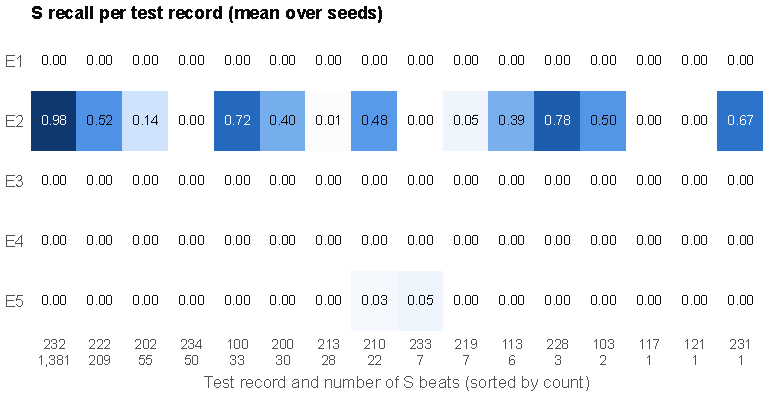
\includegraphics[width=6.3in]{figures/per_patient_S.pdf}
\caption{S sensitivity for each test record (mean over seeds), records sorted by their number of S beats (second line of the labels). E2's sensitivity in record 232 comes with S predictions for almost every beat of that record (Section 4.4).}\label{fig:3}
\end{figure}

\subsection{Failure analysis}

\textbf{Where are the errors?} For E1, two records account for 86\% of the S errors: record 232 (1,379 S beats called N, 99.9\% of its S beats) and record 222 (all 209 S beats called N). The other large error cells are record 213 (363 N beats called V; F beats split between N and V) and record 233 (202 V beats called N, 24\%).

\textbf{Did the models learn S on the training patients?} On training and validation data only, the selected checkpoints of E1, E3, E4 and two of the three E5 seeds detect at most 3\% of the S beats in their own training set. Early stopping kept epochs 1–5 in 14 of the 15 patient-split runs (epoch 9 in the other), against 18–29 for E0, because validation macro-F1 stopped improving almost at once while the validation loss of E1 rose from the first epochs (Fig.~\ref{fig:4}). The models that did fit S still fail on new patients: E2 detects 85–90\% of its training S beats and E5 (seed 42) 61\%, yet they find at most 8\% of the S beats of the validation patients. Two failures therefore stack: model selection stops before S is learned, and S learned on the training patients does not transfer.

\begin{figure}[!htb]
\centering
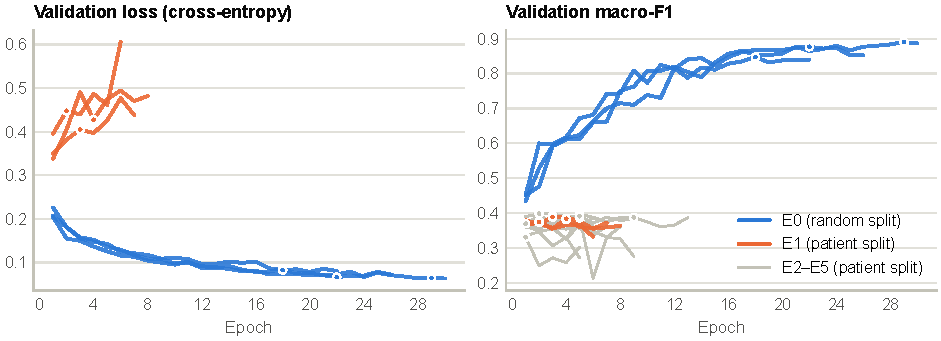
\includegraphics[width=6.3in]{figures/training_curves.pdf}
\caption{Validation loss (E0 and E1, cross-entropy) and validation macro-F1 (all experiments) per epoch; dots mark the epoch kept by early stopping. On the patient split, validation loss rises after the first epochs and macro-F1 never improves.}\label{fig:4}
\end{figure}

\textbf{E2 labels patients, not beats} \emph{(post-hoc)}. Class weighting makes E2 call 98\% of all beats in record 232 S, including 99\% of that record's 397 N beats. Because 78\% of the record's beats are S, this produces most of the S “gain”. The same behaviour produces the false positives: 92\% of the N beats of record 212 (2,530 of 2,746) are called S, as are 80\% of those of record 222 and 68\% of those of record 100. Within record 232, E2's S probability separates S from N beats no better than chance (AUROC 0.48\,±\,0.06).

\textbf{E5 ranks S beats correctly but never predicts them} \emph{(post-hoc)}. Table~\ref{tab:4} measures how well each model's S probability ranks S beats above all other beats, across all test beats pooled and within each record. Pooled AUROC looks moderate for every patient-split model (0.75–0.86), but within records E1–E4 are at or below chance (median 0.46–0.48): their pooled score separates patients, not beats. E5 is the exception. Within record 232 its S probability separates S from N almost perfectly (AUROC 0.994), and the median over records is 0.895, yet the argmax never selects S.

\begin{table}[!htb]
\centering\small
\caption{\emph{(Post-hoc.)} AUROC of the S probability for S versus all other beats, mean over seeds. Within records: median over the 8 test records with at least 10 S and 10 other beats.}\label{tab:4}
\begin{tabular}{lllll}
\toprule
\textbf{Exp} & \textbf{Pooled} & \textbf{Within records (median)} & \textbf{Within record 232} & \textbf{Share of record 232 predicted S} \\
\midrule
E0 (random split) & 0.963 & 0.943 & 0.948 & 0.775 \\
E1 & 0.753 & 0.467 & 0.429 & 0.000 \\
E2 & 0.859 & 0.478 & 0.482 & 0.983 \\
E3 & 0.863 & 0.475 & 0.461 & 0.000 \\
E4 & 0.762 & 0.457 & 0.419 & 0.000 \\
E5 & 0.863 & 0.895 & 0.994 & 0.000 \\
\bottomrule
\end{tabular}
\end{table}

\textbf{Would a better threshold fix it?} \emph{(Post-hoc; thresholds chosen on validation patients only.)} We predicted S whenever the S probability exceeded the threshold that maximised S F1 on the four validation records. For no model does this transfer. For E1, E2 and E4 the threshold labels most test beats S (S Se 0.94–1.00, +P 0.04–0.07). E3 reaches S F1 0.21\,±\,0.11, but with within-record ranking at chance this again labels patients rather than beats. For E5 the outcome depends on the seed (S Se 0.62\,±\,0.45, +P 0.11\,±\,0.05, S F1 0.15\,±\,0.08), and macro-F1 is no better than with the argmax (0.420 against 0.445). The scores are informative within a patient but not comparable between patients.

\textbf{Why does timing not transfer?} In the training set, 62\% of S beats (395 of 640) occur inside supraventricular tachycardia runs, mostly in record 209, where they are not early relative to the preceding beats. Only 48.9\% of training S beats have a prematurity index below 0.9, against 87.7\% of test S beats (Fig.~\ref{fig:5}). Within record 232, S beats correlate at r = 0.975 with that record's N beats in shape; their timing is what differs. The cue that defines most test S beats is therefore weak in training.

\begin{figure}[!htb]
\centering
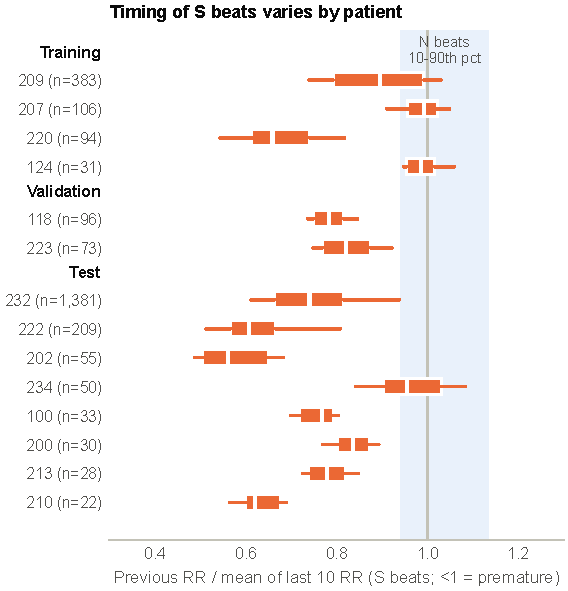
\includegraphics[width=4.0in]{figures/rr_prematurity_S.pdf}
\caption{Prematurity index of S beats per record (previous RR divided by the mean of the last ten RR intervals; below 1 means early): median, interquartile range and 10th–90th percentiles. Training records 209 and 207 have S beats that are not early; most test S beats, led by record 232, are early.}\label{fig:5}
\end{figure}

\section{Discussion and Limitations}

\textbf{The headline number depends on the split.} The same 13.5k-parameter CNN, trained in the same way, scores macro-F1 0.874 when beats are split at random and 0.429 when the test patients are new, and on new patients it detects no S or F beats. This matches the direction reported in the literature~\cite{dechazal2004automatic,Sellami2019} and shows how far the random-split number overstates what a deployed model would do.

\textbf{Why the inexpensive fixes did not recover S.} Reweighting the loss (E2) did not teach the network what an S beat looks like in a new patient; it taught the network to call whole patients S. Imbalance is real, but it is not what blocks generalisation. Augmentation (E4) simulates gain, noise and baseline changes, while the S beats of record 232 differ from its N beats in timing, not shape, so, as expected, it did not help. RR features (E5) did teach the right cue: within record 232 the network ranks S above N almost perfectly. But no test beat crosses the decision boundary, and a threshold chosen on the validation patients does not help, because S scores are not comparable between patients. The training data teach a weaker timing cue than the test patients need.

\textbf{Pooled metrics can mislead.} The gap between pooled and within-patient AUROC (0.75–0.86 against 0.46–0.48 for E1–E4) shows that a pooled ranking metric can look reasonable when a model only separates patients with many S beats from patients with few. Within-patient analysis exposes this, and we recommend reporting it alongside pooled scores.

\textbf{Model selection under patient shift.} Early stopping on validation macro-F1 chose epochs 1–5 in 14 of 15 patient-split runs, before the network had learned S even on its training patients. This is itself a symptom of the shift: learning S on the training patients did not raise validation macro-F1, because the validation patients' S beats differ. Where S was learned (E2 and one E5 seed), validation S sensitivity stayed at or below 0.08, so the failure to generalise does not depend on the early stop. Still, E3–E5 partly compare under-trained models, and a selection rule that does not rely on four validation patients would make the comparison cleaner.

\textbf{Limitations.} (i) \emph{Few patients}: 22 test patients, two of whom hold most of the S (record 232: 75\%) and F (record 213: 93\%) beats, so S and F conclusions describe a handful of individuals, and a 22-record bootstrap is itself approximate~\cite{Efron1993}. (ii) \emph{Weak validation set}: four patients with 175 S and 17 F beats guide early stopping and threshold choice. (iii) \emph{Statistics}: three seeds per configuration, SDs up to 0.155 (E2 accuracy), intervals instead of significance tests, and no correction for comparing four fixes. (iv) \emph{Data}: one lead, annotated beat locations instead of a detector, an offline next-RR feature, paced records and the Q class excluded, and no external test database. (v) \emph{Post-hoc analyses}: the ranking and threshold analyses were designed after we saw the first test results; they explain the failure and were not used to select any model.

\textbf{Future work.} The within-patient result suggests that the missing step is per-patient calibration rather than more features: normalising RR features by each patient's own rhythm, adapting the threshold with a few labelled beats from the new patient, as in patient-specific training~\cite{Kiranyaz2016}, or unsupervised test-time adaptation. Each needs a validation design with more patients, for example leave-one-patient-out on DS1.

\section{Conclusion}

On MIT-BIH, a 1D CNN that scores macro-F1 0.874 on a random beat split scores 0.429 on patients it has not seen and detects none of their S or F beats. Four inexpensive fixes did not change this. Class weighting raised S sensitivity to 0.83, but only by labelling entire patients S (S +P 0.115); focal loss and augmentation had no effect on S; RR features gave the only reliable macro-F1 gain (+0.016, through V). Their main effect was hidden: the model learned to rank S beats correctly within each patient (AUROC 0.994 in record 232) but never predicted them, and a threshold chosen on other patients did not fix this. Patient-wise evaluation should report per-patient results and within-patient ranking alongside pooled scores, because pooled scores can hide both failures and partial successes. The next step is to calibrate decisions per patient.

\section*{AI Use Statement}

We used generative AI tools in all three roles, and each member checked the output of the tool they used.

\placeholder{\textbf{[M1 to write: the tools M1 used, for what, and how the outputs were checked.]} Draft: \texttt{docs/report/M1\_AI\_USE\_DRAFT.md}.}

\placeholder{\textbf{[M2 to write: the tools M2 used (exact name and model), for what, and how the outputs were checked.]}}

M3 used Claude Code (Claude Opus 5.5) for the prediction-export, evaluation and figure code, the post-hoc analyses, reference checking and first drafts of Sections 1, 2.3, 3.5 and 4–6. The code was checked with unit tests (including cross-checks against scikit-learn), every reported number was regenerated from the code's output, and every reference was checked against the publisher, PubMed or arXiv record. [Yitian: how you reviewed and revised the text.]

Our team chose the research question, the subject-disjoint protocol and the experiments, decided how to report the early-stopping problem, and interpreted the results. Every result comes from experiments we ran.

\clearpage

\section*{References}

\printbibliography[heading=none]

\clearpage

\appendix

\renewcommand{\thefigure}{\thesection\arabic{figure}}

\renewcommand{\thetable}{\thesection\arabic{table}}

\counterwithin*{figure}{section}

\counterwithin*{table}{section}

\section{Reproducing the results}

\placeholder{\textbf{[M1 and M2 to write: the data-preparation (M1) and training (M2) commands, as in the README.]}}

The evaluation is reproduced from the repository root with:

{\raggedright\begin{itemize}
\item \texttt{python -m src.predict} exports test predictions from the committed checkpoints (CPU is enough).
\item \texttt{python -m src.evaluate summarise --reference E1} writes every table and figure in this report to \texttt{results/summary/}.
\end{itemize}\par}

\section{Autoencoder pretraining (E6)}

\placeholder{\textbf{[M1 to write (optional): E6 autoencoder pretraining, and that no supervised E6 classifier was trained, so the pretraining hypothesis is untested.]} Source: \texttt{docs/report/M1\_E6\_RESULTS.md}.}

\section{Bootstrap differences}

\begin{figure}[!htb]
\centering
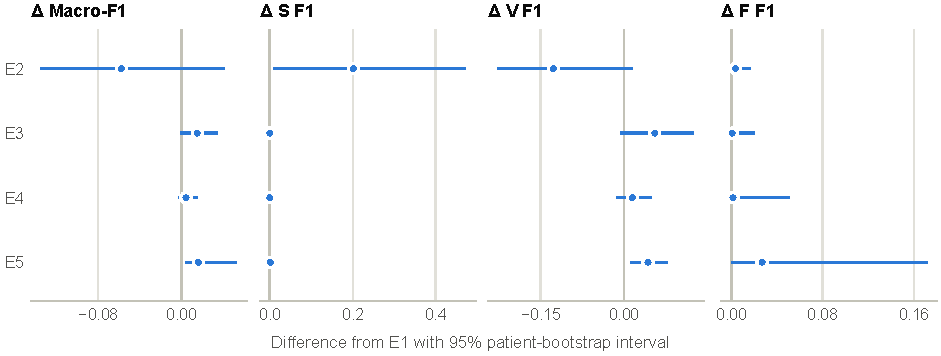
\includegraphics[width=6.3in]{figures/bootstrap_vs_reference.pdf}
\caption{Change from E1 with 95\% patient-bootstrap intervals (the data of Table~\ref{tab:3}).}\label{fig:C1}
\end{figure}

\end{document}
